\documentclass[12pt, titlepage]{article}

\usepackage{booktabs}
\usepackage{tabularx}
\usepackage{hyperref}
\hypersetup{
    colorlinks,
    citecolor=black,
    filecolor=black,
    linkcolor=red,
    urlcolor=blue
}
\usepackage{graphicx}
\usepackage{mdframed}
\usepackage{enumerate}
\usepackage[round]{natbib}
\usepackage{float}



\title{SE 3XA3: Software Requirements Specification\\Title of Project}

\author{Team 29
		\\ Ashley Williams, willia18
		\\ Declan Mullane, mullanem
		\\ Leo Shi, shiy12
}

\date{October 5, 2018}

%\input{../Comments}

\newmdenv[linecolor=black]{reqbox}


\begin{document}

\maketitle

\pagenumbering{roman}
\tableofcontents
\listoftables
\listoffigures

\begin{table}[bp]
\caption{\bf Revision History}
\begin{tabularx}{\textwidth}{llX}
\toprule {\bf Date} & {\bf Version} & {\bf Notes}\\
\midrule
Oct. 3 & Ashley Williams & Initial Draft\\
Oct. 3 & Declan Mullane & Initial Draft\\
Oct. 3 & Leo Shi & Initial Draft\\
Oct. 5 & Ashley Williams & Revision 0\\
Oct. 5 & Declan Mullane & Revision 0\\
Oct. 5 & Leo Shi & Revision 0\\
\bottomrule
\end{tabularx}
\end{table}

\newpage

\pagenumbering{arabic}

%This document describes the requirements for Garden Defenders. The template for the Software
%Requirements Specification (SRS) is a subset of the Volere
%template~\citep{RobertsonAndRobertson2012}.  If you make further modifications
%to the template, you should explicitly state what modifications were made.

\section{Project Drivers}

\subsection{The Purpose of the Project}

This project aims to re-implement Game1, a downloadable shooter game, to make it accessible via web browser. Through this re-implementation, the project aims to alleviate boredom and provide entertainment on a new platform for a wider range of people.  

\subsection{The Stakeholders}

\subsubsection{The Client}

We are both client and customer for this project. The goal we would like to see realized is for Game1 to be brought to a larger audience through the medium of web browsers. 

\subsubsection{The Customers}

The client and customer for this project are the same.

\subsubsection{Other Stakeholders}

Other stakeholders of the project include the users, or players, who will consumer our game after it is finished. These may include experienced and inexperienced players. The age range for the players is 7+, for content as well as difficulty. 

Play testers will also be consulted before the project is finished to ensure other people are able to learn how to play the game, to ensure its functionality, and to measure user reactions for game satisfaction requirements. 

\subsection{Mandated Constraints}

\subsubsection{Solution Constraints}

Description: The game will be accessible on all browsers that support JavaScript. 
Rationale: JavaScript is a useful language for browser based games and will be supported on a multitude of browsers, increasing the number of players who can access the game. 
Fit Criterion: The game runs properly in all browsers that support JavaScript. 

\subsubsection{Implementation Environment of Current System}

The user will interact with their PC, which will interact with the browser running the game. 
\subsubsection{Anticipated Workplace Environment}

Anywhere the user is able to access a computer with an Internet connection is a possible environment for the project. 

\subsubsection{Schedule Constraints}

The game and its documentation will be completed on or before December 5th, 2018, as specified by the client. 

\subsection{Naming Conventions and Terminology}

\begin{table}[H]
    \caption{Naming Conventions and Terminology}
    \centering
    \begin{tabular}{c|c}
         \bf Term & \bf Meaning \\
         \hline 
         JavaScript & Programming language used to build game \\
         Player & User playing the game \\
         Player character & The user's avatar \\
         Enemy & The non-player avatars \\
         Projectile & Weapon projectile to make attacks in game \\
         FR & Functional Requirements \\
         NFR & Non-Functional Requirements \\ 
         Health Bar & Displays how many health points the player has left until they lose \\
         Game State & The stored state of the game \\
         Defensive Line & The border the enemy crosses that reduces player health points \\
         GUI & Graphical User Interface \\
         Level & The different stages of progression in the game \\
    \end{tabular}

    \label{tab:my_label}
\end{table}
\subsection{Relevant Facts and Assumptions}

To play the game, the user must have a computer, keyboard, mouse, and monitor. Player character movement is determined by keys on the keyboard, while the trajectory and firing of weapons is controlled by the mouse. A monitor is required to view the game. An Internet connection is also required to play the game, and it is assumed that any browser the user plays the game in will be able to support JavaScript and graphics.  

\section{Functional Requirements}

\subsection{The Scope of the Work and the Product}
\subsubsection{The Current Situation}
\textbf{Content} \\
\noindent The current product is a simple Python point-and-shoot game that must be downloaded and compiled in order to be played. \\

\noindent \textbf{Motivation} \\
We want to re-implement this in JavaScript as a web browser game, so that it can be more easily enjoyed by a wider audience. We also wish to make some minor improvements, such as adding a user guide to explain how to play the game, as well as introducing levels in an effort to add complexity and hopefully keep users engaged for longer. 

\subsubsection{The Context of the Work}
\begin{figure}[H]
    \centering
    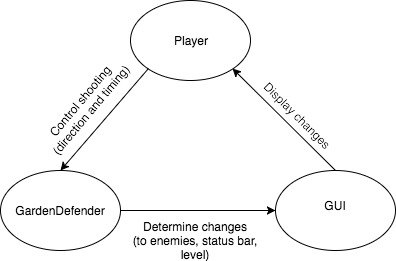
\includegraphics{context_rough.jpg}
\end{figure}

\subsubsection{Work Partitioning}
BUC Cases do not apply.

\subsubsection{Individual Product Use Cases}
\begin{table}[H]
    \caption{Individual Product Use Cases} 
    \begin{center}
       \begin{tabular}{p{0.3\linewidth} | c | p{0.5\linewidth}}
        \textbf{Use Case} & \textbf{Inputs/Outputs} & \textbf{Summary} \\
        \hline
        1. New Game & Mouse click (in) & New game is started \\
                    & Gamestate (out)  &\\
        \hline
        2. Player moves & Keyboard (in) & Player character moves accordingly in GUI \\
                        & Gamestate (out) & \\
        \hline
        3. Player shoots & Mouse click (in) & Player aims and shoots at enemies, projectiles move appropriately in GUI \\
                         & Gamestate (out) &\\
        \hline
        4. Player misses, enemy has not reached defensive line & Gamestate (out) & Enemy remains in GUI and continues in its normal path\\
        \hline
        5. Player misses, enemy surpasses defensive line & Gamestate (out) & Enemy disappears after passing defensive line, health bar decreases \\
        \hline
        6. Player hits & Gamestate (out) & Health bar remains same, enemy disappears, points increase \\
        \hline
        7. Player beats level & Gamestate (out) & Player moves onto next level \\
        \hline
        8. Player loses level & Gamestate (out) & Player brought back to new game screen \\
        \hline
        9. Player beats last level & Gamestate (out) & End screen displayed in GUI \\
        \hline
        10. Pause game & Mouse click (in) & Players selects pause, game is paused \\
                      & Gamestate (out)  & \\
        \hline
        11. Resume game & Mouse click (in) & Player selects resume, game is resumed \\
                        & Gamestate (out) &\\
        \hline
        12. Restart game & Mouse click (in) & Player brought back to new game screen \\
                        & Gamestate (out)  &\\
        \hline
        13. Toggle user guide & Mouse click (in) & Displays game instructions \\
                              & Gamestate (out)  &\\
        \end{tabular}
    \end{center}
\end{table}

\subsection{Functional Requirements}

%Requirement Box formatting template adapted from: 
%https://github.com/KelvinKKLin/GrateBox/tree/master/Documentation/SRS

\begin{reqbox}
	%
	\begin{tabular}{c|c|c}
		Requirement \#: FR-01 & Requirement Type: Functional & Use Case:10 \\
	\end{tabular} \\
	%
	\textbf{Description:} A clear and unambiguous user guide is provided along with the game. \\
	\textbf{Rationale:}  Clear instructions are essential for user understanding and success in the game. \\
	\textbf{Fit Criterion:} No play testers report being confused about how to play the game. \\
	\textbf{History:} Created October 3 2018
	%
\end{reqbox}

\begin{reqbox}
	%
	\begin{tabular}{c|c|c}
		Requirement \#: FR-02 & Requirement Type: Functional & Use Case:1 \\
	\end{tabular} \\
	%
	\textbf{Description:} New game is started when player selects new game option. \\
	\textbf{Rationale:} Cannot play game without first starting a game. \\
	\textbf{Fit Criterion:} When new game option is selected, a new initial game state is created (level 1, full health bar, 0 points). \\
	\textbf{History:} Created October 3 2018
	%
\end{reqbox}

\begin{reqbox}
	%
	\begin{tabular}{c|c|c}
		Requirement \#: FR-03 & Requirement Type: Functional & Use Case:2 \\
	\end{tabular} \\
	%
	\textbf{Description:} Player can move player character up and down the defensive line with the keyboard keys. \\
	\textbf{Rationale:}  Player character should be movable for tactical positioning. \\
	\textbf{Fit Criterion:} When the associated keyboard key is pressed for "up" or "down," the player character's coordinates change accordingly and is displayed in the GUI. \\
	\textbf{History:} Created October 3 2018
	%
\end{reqbox}

\begin{reqbox}
	%
	\begin{tabular}{c|c|c}
		Requirement \#: FR-04 & Requirement Type: Functional & Use Case:2 \\
	\end{tabular} \\
	%
	\textbf{Description:} Player character cannot be moved out of bounds. \\
	\textbf{Rationale:}  Player character should be visible in the GUI at all times. \\
	\textbf{Fit Criterion:} If the player character reaches the top or bottom boundary, it remains at the respective boundary (i.e. cannot leave the GUI). \\
	\textbf{History:} Created October 3 2018
	%
\end{reqbox}

\begin{reqbox}
	%
	\begin{tabular}{c|c|c}
		Requirement \#: FR-05 & Requirement Type: Functional & Use Case:3 \\
	\end{tabular} \\
	%
	\textbf{Description:} Player can aim and shoot. \\
	\textbf{Rationale:} Player must be able to shoot its enemies in order to progress in the game. \\
	\textbf{Fit Criterion:} When the player shoots, a projectile is displayed immediately after firing with the correct input trajectory. \\
	\textbf{History:} Created October 3 2018
	%
\end{reqbox}

\begin{reqbox}
	%
	\begin{tabular}{c|c|c}
		Requirement \#: FR-06 & Requirement Type: Functional & Use Case:4 \\
	\end{tabular} \\
	%
	\textbf{Description:} Enemies remain on display when missed. \\
	\textbf{Rationale:} If projectile misses the enemy, it has not been eliminated. \\
	\textbf{Fit Criterion:} Enemy remains in GUI, continues in its normal path. \\
	\textbf{History:} Created October 3 2018
	%
\end{reqbox}

\begin{reqbox}
	%
	\begin{tabular}{c|c|c}
		Requirement \#: FR-07 & Requirement Type: Functional & Use Case:5 \\
	\end{tabular} \\
	%
	\textbf{Description:} If enemy surpasses defensive line, enemy disappears and health bar decreases. \\
	\textbf{Rationale:} The defensive line is a boundary of the game, so the enemy will become out of bounds and should disappear; the player character is damaged when an enemy passes it. \\
	\textbf{Fit Criterion:} Enemy's coordinates on grid are registered as out of bounds/surpassing defensive line, enemy disappears from display and health bar decreases accordingly. \\
	\textbf{History:} Created October 3 2018
	%
\end{reqbox}

\begin{reqbox}
	%
	\begin{tabular}{c|c|c}
		Requirement \#: FR-08 & Requirement Type: Functional & Use Case:6 \\
	\end{tabular} \\
	%
	\textbf{Description:} When an enemy is hit, the enemy disappears and the player's points increase by 1. \\
	\textbf{Rationale:} Eliminating enemies is how the player progresses and earns points. \\
	\textbf{Fit Criterion:} Projectile coordinates and enemy coordinates intersect, enemy disappears and the player's points increase by 1. \\
	\textbf{History:} Created October 3 2018
	%
\end{reqbox}

\begin{reqbox}
	%
	\begin{tabular}{c|c|c}
		Requirement \#: FR-09 & Requirement Type: Functional & Use Case:7 \\
	\end{tabular} \\
	%
	\textbf{Description:} When the player collects enough points to beat the level, they proceed to the next level. \\
	\textbf{Rationale:} Object of the game is to beat all levels without losing all health points. \\
	\textbf{Fit Criterion:} When the player collects the required amount of points for a certain level, the next level screen is displayed. \\
	\textbf{History:} Created October 3 2018
	%
\end{reqbox}

\begin{reqbox}
	%
	\begin{tabular}{c|c|c}
		Requirement \#: FR-10 & Requirement Type: Functional & Use Case:8 \\
	\end{tabular} \\
	%
	\textbf{Description:} When the player loses a level, they are brought back to the new game screen. \\
	\textbf{Rationale:} In order to beat the game, all levels must be passed consecutively. \\
	\textbf{Fit Criterion:} When the player's health bar reaches zero, they are brought back to the new game screen. \\
	\textbf{History:} Created October 3 2018
	%
\end{reqbox}

\begin{reqbox}
	%
	\begin{tabular}{c|c|c}
		Requirement \#: FR-11 & Requirement Type: Functional & Use Case:9 \\
	\end{tabular} \\
	%
	\textbf{Description:} If the player beats the last level, the game has been beaten. \\
	\textbf{Rationale:} The last level is the end of the game. \\
	\textbf{Fit Criterion:} When the player collects the required amount of points for the last level, the end screen is displayed in the GUI. \\
	\textbf{History:} Created October 3 2018
	%
\end{reqbox}

\begin{reqbox}
	%
	\begin{tabular}{c|c|c}
		Requirement \#: FR-12 & Requirement Type: Functional & Use Case:10 \\
	\end{tabular} \\
	%
	\textbf{Description:} Player can pause the game. \\
	\textbf{Rationale:} Player may have to temporarily pause the game. \\
	\textbf{Fit Criterion:} When the player selects the pause option, the state of the game is "frozen" (no changes in enemy position, projectile position, health bar or player points). \\
	\textbf{History:} Created October 3 2018
	%
\end{reqbox}

\begin{reqbox}
	%
	\begin{tabular}{c|c|c}
		Requirement \#: FR-13 & Requirement Type: Functional & Use Case:11 \\
	\end{tabular} \\
	%
	\textbf{Description:} Player can resume game. \\
	\textbf{Rationale:} After pausing game, player may eventually want to resume. \\
	\textbf{Fit Criterion:} When the player selects the resume option, the state of the game continues from its "frozen" state (enemies and projectiles resume movement). \\
	\textbf{History:} Created October 3 2018
	%
\end{reqbox}

\begin{reqbox}
	%
	\begin{tabular}{c|c|c}
		Requirement \#: FR-13 & Requirement Type: Functional & Use Case:12 \\
	\end{tabular} \\
	%
	\textbf{Description:} Player can restart the game. \\
	\textbf{Rationale:} Player may want to restart the game depending on their performance. \\
	\textbf{Fit Criterion:} When the player selects the restart option, they are brought back to the new game screen. \\
	\textbf{History:} Created October 3 2018
	%
\end{reqbox}

\section{Non-functional Requirements}

\subsection{Look and Feel Requirements}

\begin{reqbox}
	%
	\begin{tabular}{cc}
		Requirement \#: NFR-01 & Requirement Type: Non-Functional \\
	\end{tabular} \\
	%
	\textbf{Description:} All images used in Garden Defender are visually pleasing and give the game a "fresh" look. \\
	\textbf{Rationale:}  The images gives user their first impression on our game. \\
	\textbf{Originator:} Leo Shi\\
	\textbf{Fit Criterion:} No negative feedback on images received in the
questionnaire.\\
	\textbf{Supporting Materials:} HTML & CSS \\
	\textbf{History:} Created October 3 2018
	%
\end{reqbox}

\subsection{Usability and Humanity Requirements}
\subsubsection{Ease of Use Requirements}

\begin{reqbox}
	%
	\begin{tabular}{cc}
		Requirement \#: NFR-02 & Requirement Type: Non-Functional \\
	\end{tabular} \\
	%
	\textbf{Description:} Garden Defender should be easy to play for players aged 7 and older. \\
	\textbf{Rationale:}  A game that is too hard to play can easily drive players away.\\
	\textbf{Originator:} Leo Shi\\
	\textbf{Fit Criterion:} No play tester should report the game being excessively difficult to play, especially in the earliest levels. \\
	\textbf{Supporting Materials:} JavaScript \\
	\textbf{History:} Created October 3 2018
	%
\end{reqbox}

\subsubsection{Internationalization Requirements}
\begin{reqbox}
	%
	\begin{tabular}{cc}
		Requirement \#: NFR-03 & Requirement Type: Non-Functional \\
	\end{tabular} \\
	%
	\textbf{Description:} All the messages displayed must be in English. \\
	\textbf{Rationale:}  English is one of the most prevalent spoken languages in the world.\\
	\textbf{Originator:} Leo Shi\\
	\textbf{Fit Criterion:} Play testers report that English text is easy to read and comprehend. \\
	\textbf{Supporting Materials:} Google Translator \\
	\textbf{History:} Created October 3 2018
	%
\end{reqbox}

\subsection{Performance Requirements}

\subsubsection{Speed and Latency Requirements}
\begin{reqbox}
	%
	\begin{tabular}{cc}
		Requirement \#: NFR-04 & Requirement Type: Non-Functional \\
	\end{tabular} \\
	%
	\textbf{Description:} The game should be launched rapidly. \\
	\textbf{Rationale:}  Taking too long to launch will lead to players' loss of patience.\\
	\textbf{Originator:} Leo Shi\\
	\textbf{Fit Criterion:} No test case indicates that the game takes more than 5 seconds to launch.\\
	\textbf{Supporting Materials:} JavaScript \\
	\textbf{History:} Created October 3 2018
	%
\end{reqbox}


\subsubsection{Reliability and Availability Requirements}
\begin{reqbox}
	%
	\begin{tabular}{cc}
		Requirement \#: NFR-05 & Requirement Type: Non-Functional \\
	\end{tabular} \\
	%
	\textbf{Description:} The game should be able to run all the time. \\
	\textbf{Rationale:} A game that crashes often will lose its players.\\
	\textbf{Originator:} Leo Shi\\
	\textbf{Fit Criterion:} No test case indicates that the game ever crashes.\\
	\textbf{Supporting Materials:} JavaScript \\
	\textbf{History:} Created October 3 2018
	%
\end{reqbox}

\subsection{Operational and Environmental Requirements}

\subsubsection{Expected Physical Environment}
\begin{reqbox}
	%
	\begin{tabular}{cc}
		Requirement \#: NFR-06 & Requirement Type: Non-Functional \\
	\end{tabular} \\
	%
	\textbf{Description:} The game should be able to run on any computer with a web browser.\\
	\textbf{Rationale:} Players will play our game using those devices.\\
	\textbf{Originator:} Leo Shi\\
	\textbf{Fit Criterion:} No test case indicates that the game fails to run on any modern computer.\\
	\textbf{Supporting Materials:} JavaScript \\
	\textbf{History:} Created October 3 2018
	%
\end{reqbox}

\subsubsection{Requirements for Interfacing with Adjacent Systems}
\begin{reqbox}
	%
	\begin{tabular}{cc}
		Requirement \#: NFR-07 & Requirement Type: Non-Functional \\
	\end{tabular} \\
	%
	\textbf{Description:} The game should be able to run on most major web browsers. \\
	\textbf{Rationale:} Players will play our game using web browsers.\\
	\textbf{Originator:} Leo Shi\\
	\textbf{Fit Criterion:} The game successfully runs on over 80 percent of major web browsers selected in our test case.\\
	\textbf{Supporting Materials:} JavaScript \\
	\textbf{History:} Created October 3 2018
	%
\end{reqbox}

\subsection{Maintainability and Support Requirements}

\subsubsection{Adaptability Requirements}
\begin{reqbox}
	%
	\begin{tabular}{cc}
		Requirement \#: NFR-08 & Requirement Type: Non-Functional \\
	\end{tabular} \\
	%
	\textbf{Description:} The game should be able to run on Windows, Apple, and Linux.\\
	\textbf{Rationale:} Windows, Apple, and Linux are the most commonly used operating systems for our users.\\
	\textbf{Originator:} Leo Shi\\
	\textbf{Fit Criterion:} No test case indicates our game fails to operate on any of those operating systems.\\
	\textbf{Supporting Materials:} JavaScript \\
	\textbf{History:} Created October 3 2018
	%
\end{reqbox}

\subsection{Security Requirements}
Security Requirements are not applicable to our project.

\subsection{Cultural Requirements}
\begin{reqbox}
	%
	\begin{tabular}{cc}
		Requirement \#: NFR-09 & Requirement Type: Non-Functional \\
	\end{tabular} \\
	%
	\textbf{Description:} The game will include no text or images of an offensive nature to any groups that may play the game. \\
	\textbf{Rationale:} Fun games should be inclusive to all consumers, and producing an offensive game could lose players. \\
	\textbf{Originator:} Declan Mullane\\
	\textbf{Fit Criterion:} After surveying players, more than 95\% of players should find the game unoffensive. \\
	\textbf{Supporting Materials:}  N/A\\
	\textbf{History:} Created October 5 2018
	%
\end{reqbox}
\subsection{Legal Requirements}

Legal Requirements are not applicable to our project.

\subsection{Health and Safety Requirements}

\begin{reqbox}
	%
	\begin{tabular}{cc}
		Requirement \#: NFR-10 & Requirement Type: Non-Functional \\
	\end{tabular} \\
	%
	\textbf{Description:} The game must not cause any physical or mental distress to the players.\\
	\textbf{Rationale:} Health and safety are crucial and therefore should be considered with a high priority in our project.\\
	\textbf{Originator:} Leo Shi\\
	\textbf{Fit Criterion:} No play testers should report physical or mental discomfort as a result of our game. \\
	\textbf{Supporting Materials:} N/A \\
	\textbf{History:} Created October 3 2018
	
\end{reqbox}

\section{Project Issues}

\subsection{Open Issues}
Some issues with the current game including:

\begin{itemize}
\item With only one character and one stage design, the game is unable to hold interest for long.
\item Its default difficulty exceeds the average player's capabilities.
\item The game lacks any form of instruction, which makes it unfriendly to users.
\item The game was not very portable as it requires the python shell to run.
\end{itemize}

\subsection{Off-the-Shelf Solutions}
Many similar open source shooting games written in JavaScript are available on the Internet. Components in those games, along with the convenient functions in some JavaScript game engines, will be considered as Off-the-Shelf solutions in order to save development time.

\subsection{New Problems}
Currently there are no new problem. This will be updated if new problems are found when we proceed further into the project.

\subsection{Tasks}
\begin{center}
\begin{table}[H]
    \caption{Tasks} 
    \begin{tabular}{|c|c|}
	\hline
	Tasks & Timeline \\ \hline
	Rebuild the game using JavaScript  & Oct 18, 2017 \\ \hline
	Adding features and adjusting difficulty & Oct 20, 2017 \\ \hline
	Finish web page interface & Oct 22, 2017 \\ \hline
	Finish test cases & Oct 24, 2017 \\ \hline
	Finish documentation & Nov 10, 2017 \\ \hline
	Final Demonstration & Nov 27, 2017 \\ \hline
    \end{tabular}
\end{table}
\end{center}

\subsection{Migration to the New Product}
Not applicable to our project.

\subsection{Risks}
The most likely risk for our project would be falling behind schedule and, as a consequence, finding time to make up lost time. 

\subsection{Costs}
There will be no cost as all software we used is free and no external hardware is required for our project.

\subsection{User Documentation and Training}
No training is required for our project. An instruction on game controls will be provided on the game web page. A thorough game tutorial will be created if our test case indicates that over 50\% of players have difficulty understanding our instructions.

\subsection{Waiting Room}
Not applicable to our project.

\subsection{Ideas for Solutions}
Learn more about test cases and check test cases for some other game projects.

\bibliographystyle{plainnat}

\bibliography{SRS}

\newpage

\section{Appendix}

This section has been added to the Volere template.  This is where you can place
additional information.

\subsection{Symbolic Parameters}

The definition of the requirements will likely call for SYMBOLIC\_CONSTANTS.
Their values are defined in this section for easy maintenance. 


\end{document}